\newpage

\section{Natural Frequency and Damping of a Second Order System and Issues with Aliasing}
\label{s:pendulum}

\subsection{Parts List}

\begin{enumerate}[itemsep=-5pt]
\item Laptop
\item CPX/CPB
\item USB Cable
\item Some sort of oscillating system like a swinging pendulum or vibrating ruler
\end{enumerate}

\subsection{Learning Objectives}
\begin{enumerate}[itemsep=-5pt]
\item Learn the basic form of a second order system
\item Understand the difference between underdamped, critically damped, and overdamped
\item Understand natural frequency and damping ratio
\item Applied Estimation of a Second Order system
\item Understand the pitfalls of aliasing
\end{enumerate}

\subsection{Getting Started}
A second order system undergoing free motion will have dynamics that look like this
\begin{equation}
\ddot{\theta} + 2\zeta \omega_n \dot{\theta} + {\omega_n}^2
\end{equation}

In this case, the solution to the above equation can be solved using \href{https://www.youtube.com/watch?v=VOv2HI3i7oo}{standard second order differential equation techniques} to obtain the solution below.
\begin{equation}\label{e:secondorder}
\theta(t) = \theta_0e^{-\sigma t}cos(\omega_d t)
\end{equation}
\begin{equation}
\omega_n = \sqrt{\sigma^2 + {\omega_d}^2}
\end{equation}
\begin{equation}
\zeta = \frac{\sigma}{\omega_n}
\end{equation}
Looking at the equations you can see that if the time series of the oscillations are known, the damping constant and damped natural frequency can be obtained. These two values can be combined to obtain the natural frequency and the damping ratio. So let’s get some data. 

\subsection{Oscillatory Ideas}

What I’d like you to do for this lab is to find some sort of parameter that varies in some sort of sinusoidal way. I’ve come up with a few ideas below. You may pick anyone you want although some are easier than others.

\begin{enumerate}[itemsep=-5pt]
\item Drive over a speed bump - If you drive over a speed bump slowly and place your CPX on the dashboard your car will hopefully vibrate for a few seconds after you drive over it. Your acceleration will look somewhat like a sine wave.
\item Vibrate a ruler - If you place a ruler on the edge of a desk and deflect it, it will vibrate. If you place the CPX on the ruler you’ll be able to measure the vibration of the ruler.
\item Attach CPX to a spring or a weight to the end of rubber bands - Take the CPX and attach it to a weight of some kind and attach the weight to a spring or a set of rubber bands. This is a mass spring damper simple and will vibrate at the natural frequency of square root of stiffness divided by mass. I chose to do this example.
\item Build a Pendulum: If you decide to build a pendulum, you need to hang a weight on the CPX or attach the CPX to something heavy. This will make the ratio between cable to end mass much smaller and thus better for data and fitting. An example includes  duct taping your CPX to a water bottle or something. It would also be better to use a string and mount the CPX to the string with an external battery pack and have the CPX log data internally. This way most of the mass would be concentrated at the tip of the pendulum. Another idea is to take a paper towel cardboard tube and tape the cpx inside it with the cable running through it. Then duct a large weight on the end of the paper towel tube and then hinge the top of the tube by skewering a screwdriver through it. This will allow the tube to swing like a pendulum rather than the string. 
\end{enumerate}
There are most likely many other options so try and get creative and find something oscillatory or dynamic in some way. Try to find something that changes relatively quickly. The temperature outside changes in a sinusoidal fashion but it’s so slow it would take you days to do this experiment. 

\subsection{Pendulum Example}

In this example I'm going to swing a pendulum in the X/Y plane of the accelerometer sensor so that I can ignore the Z axis data. I'm going to get the actual angle of the pendulum but if you're building something else you can ignore this part. You’ll notice that when you point the CPX directly at you with the cable pointing up the x axis reads around 0 and the y axis reads around gravity. If you then rotate the sensor so that the cable is coming out of the left side of the CPX, the x axis is reading about gravity while the y axis is zero. This means we can form a triangle and get the angle using these two axes using the equation below which gives angle in degrees.
\begin{equation}
\theta = tan^{-1}(x/y)\frac{180}{\pi}
\end{equation}
On the CPX specifically we want to import the math module and use the atan2 function. When I swing the pendulum then this is the result I get from Plotter in Mu.
\begin{figure}[H]
  \begin{center}
    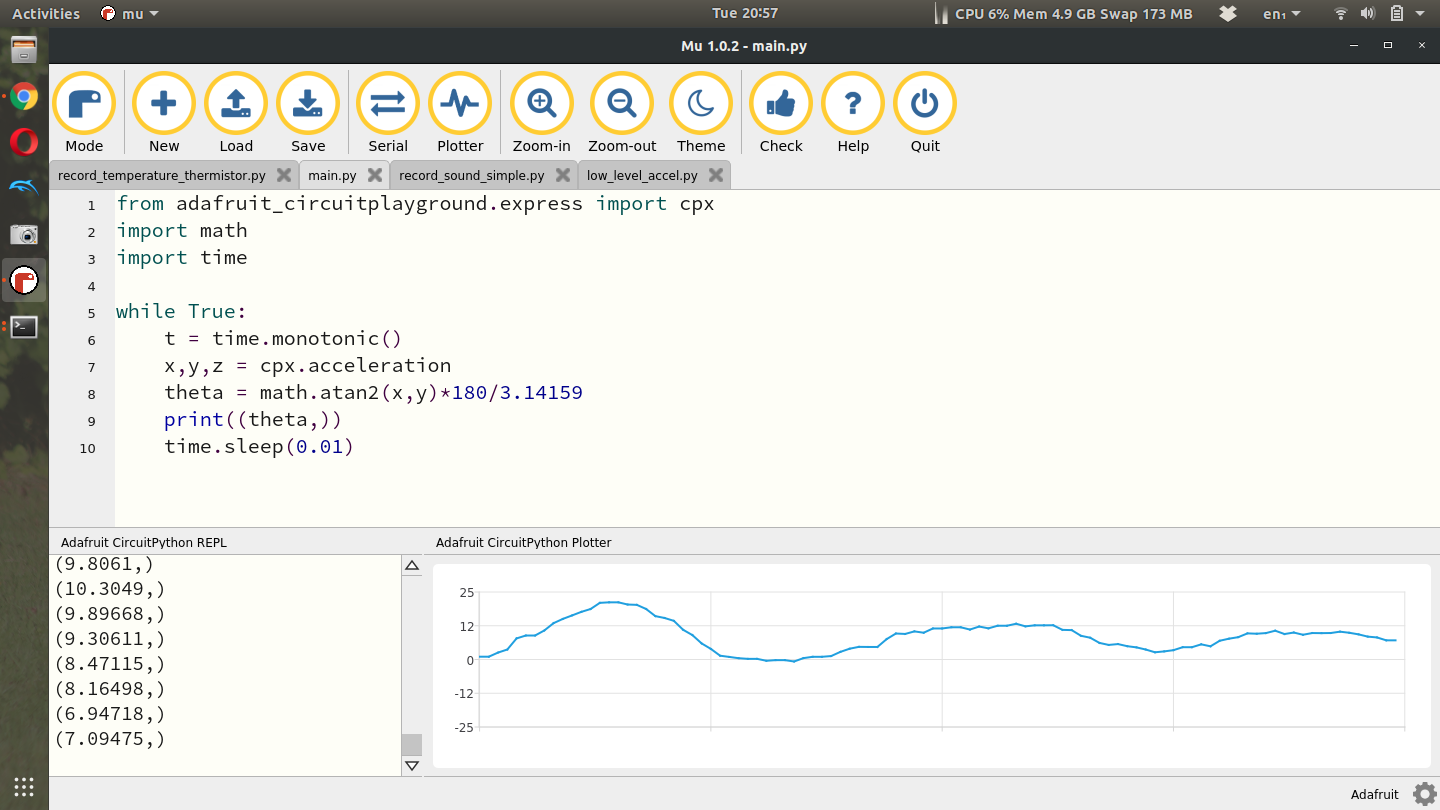
\includegraphics[width=\textwidth]{Figures/oscillation_mu.png}
  \end{center}
\end{figure}
If I then bring this into Python I get the following plot below. In my data set I only logged the angle. Since the time step between each point was 0.01 seconds I was able to just create a time series. It’s pretty clear that there is some nonlinearity in the data so I chose to start the data at 0.5 seconds. Another thing I noticed was that the angle settled out to around 8 degrees so I chose to subtract off that bias from the angle data.
\begin{figure}[H]
  \begin{center}
    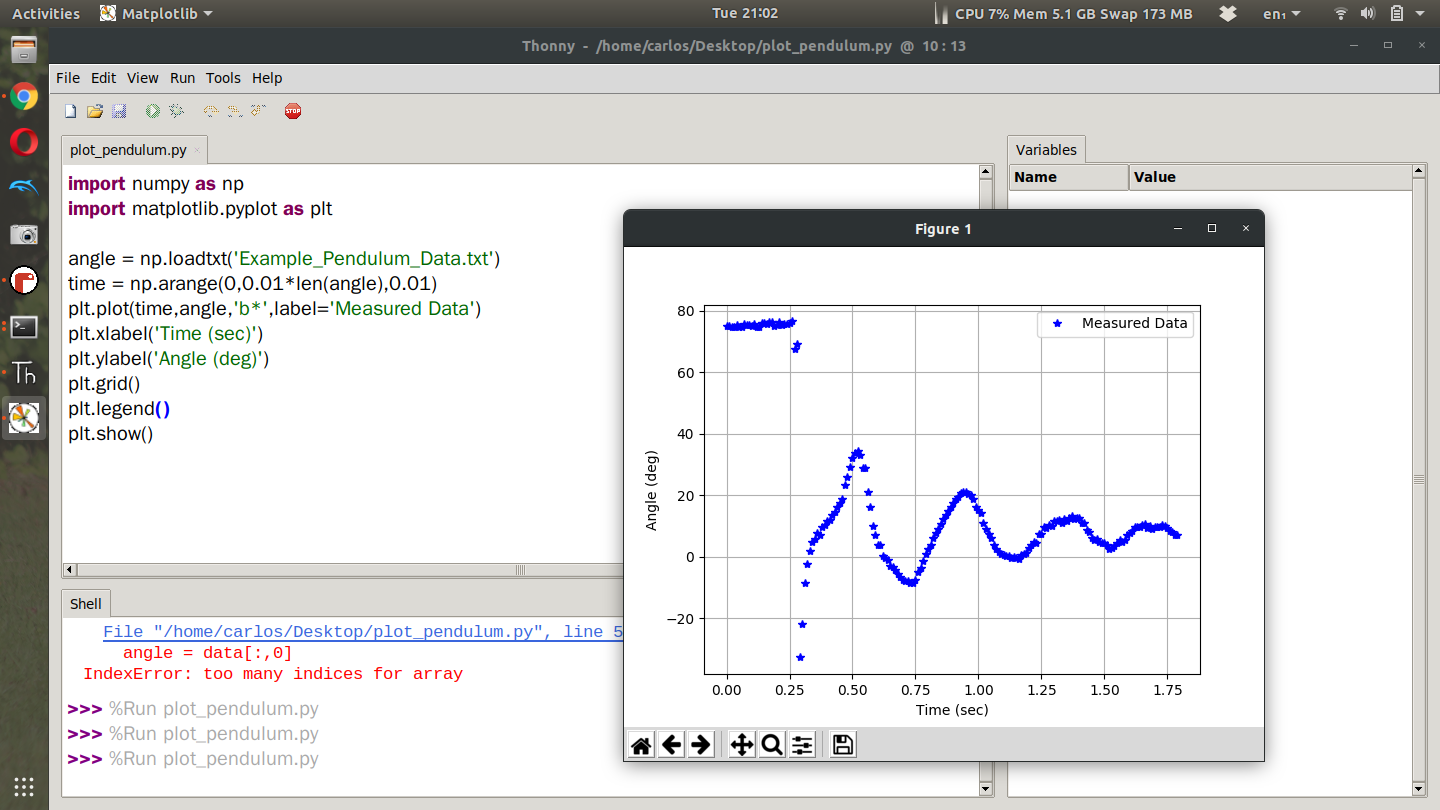
\includegraphics[width=\textwidth]{Figures/oscillation_plots.png}
  \end{center}
\end{figure}
After trimming the data and removing some bias it was time to get my damping constant and damped natural frequency. There are a few equations that can help you obtain these parameters. First, the settling time is the length of time it takes for the oscillations to settle. The settling time can be used to find the damping constant. This is equal to:
\begin{equation}
\sigma = \frac{4}{T_s}
\end{equation}
For my data set the settling time was about 1.25 seconds which gave a damping constant of 3.2. Once I had the damping constant I could obtain the damped natural frequency. This was done by measuring the distance between two peaks in the data set. There is a peak at around 0.5 seconds and another at around 0.95 seconds. I can use this to compute a period T. Period can be computed to angular frequency using the equation below.
\begin{equation}
\omega_d = \frac{2\pi}{T}
\end{equation}
Using the period in my wave form I obtained a damped natural frequency of about 14.8 rad/s. Using these values I can plot the simulated data on top of the measured data noting that my initial angle was about 35 degrees minus the bias of 8 degrees. When I first plotted the data I noticed that my fit wasn’t entirely perfect. My period was correct but my damping rate was too high. I realized it was because my settling time was too big. I increased the settling time to 1.8 seconds and got this plot here. You can see that my fitted data lined up almost perfectly with my measured data.
\begin{figure}[H]
  \begin{center}
    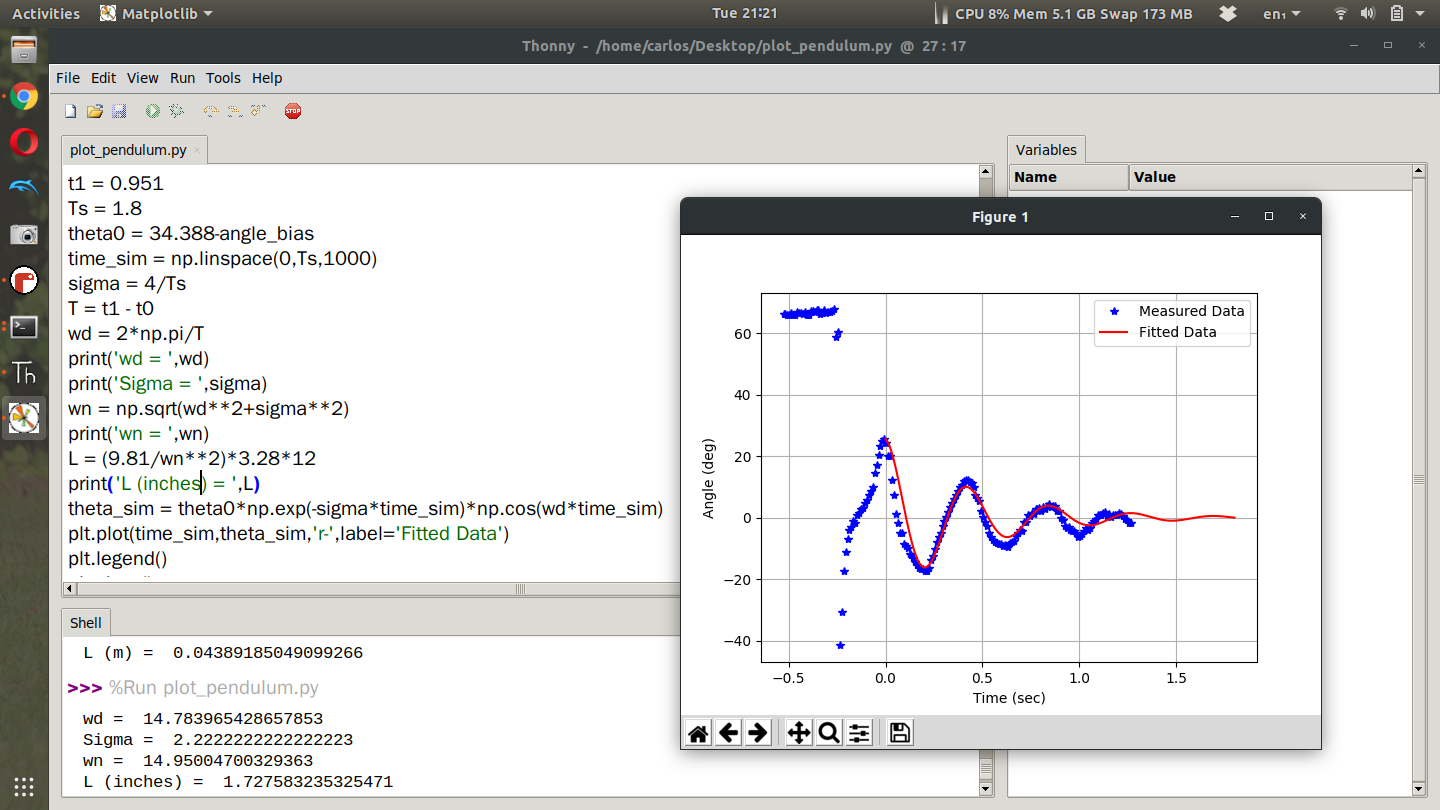
\includegraphics[width=\textwidth]{Figures/oscillation_plots2.png}
  \end{center}
\end{figure}
\subsection{Aliasing}
Aliasing occurs when you don't take data fast enough. The speed of taking data to avoid aliasing depends on the natural frequency of the system itself. To show this I changed the length of the pendulum which changed the natural frequency. I then proceeded to measure the angle as it oscillated at its natural frequency. I repeated this at sampling frequencies of 1, 10 and 100 Hz. The way I changed the sampling frequency was by changing the time.sleep value in the while True loop. The \href{https://github.com/cmontalvo251/Microcontrollers/blob/master/Circuit_Playground/CircuitPython/Accelerometer/low_level_accel.py}{accelerometer code} I used can be found on Github. After I finished the experiment I had 3 data files that I plotted on top of each other. This what I got with the longest string. It’s easy to see in the photo that sampling at 1 Hz was way too slow to capture the natural oscillations of the water bottle. However, 100 Hz and even 10 Hz was plenty fast to sample the oscillations. According to the recorded data there was above 19 cycles in 9 seconds which is about 2 Hz. In this case, as long as we sample at 4 Hz the signal will be captured properly which is why 10 Hz and 100 Hz is able to capture the signal correctly.
\begin{figure}[H]
  \begin{center}
    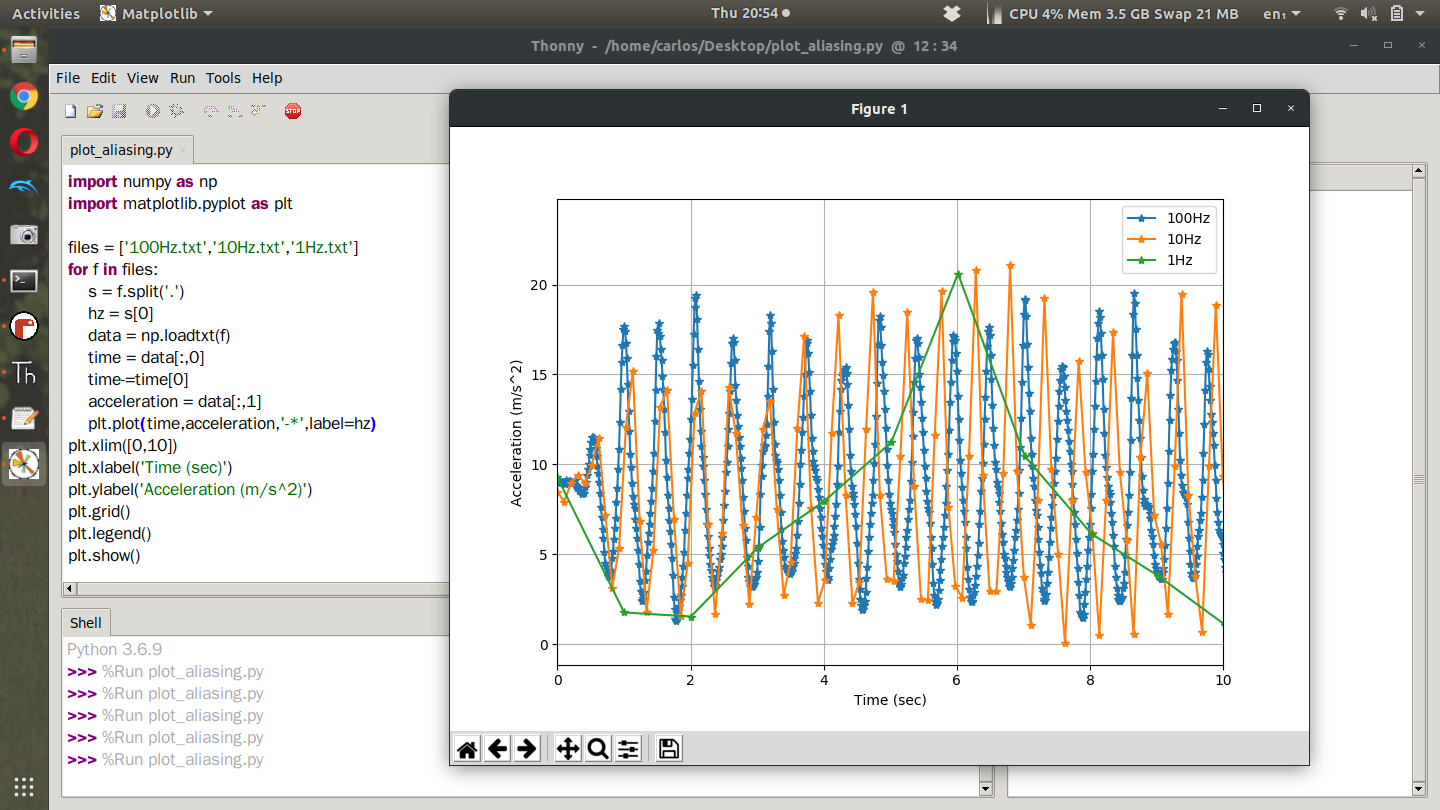
\includegraphics[width=\textwidth]{Figures/aliasing.png}
  \end{center}
\end{figure}
Once I sampled my waveform at 3 different sampling rates I elected to shrink the length of the pendulum to change the natural frequency and see if that affected any aliasing I saw. The results are shown in the figure below.
\begin{figure}[H]
  \begin{center}
    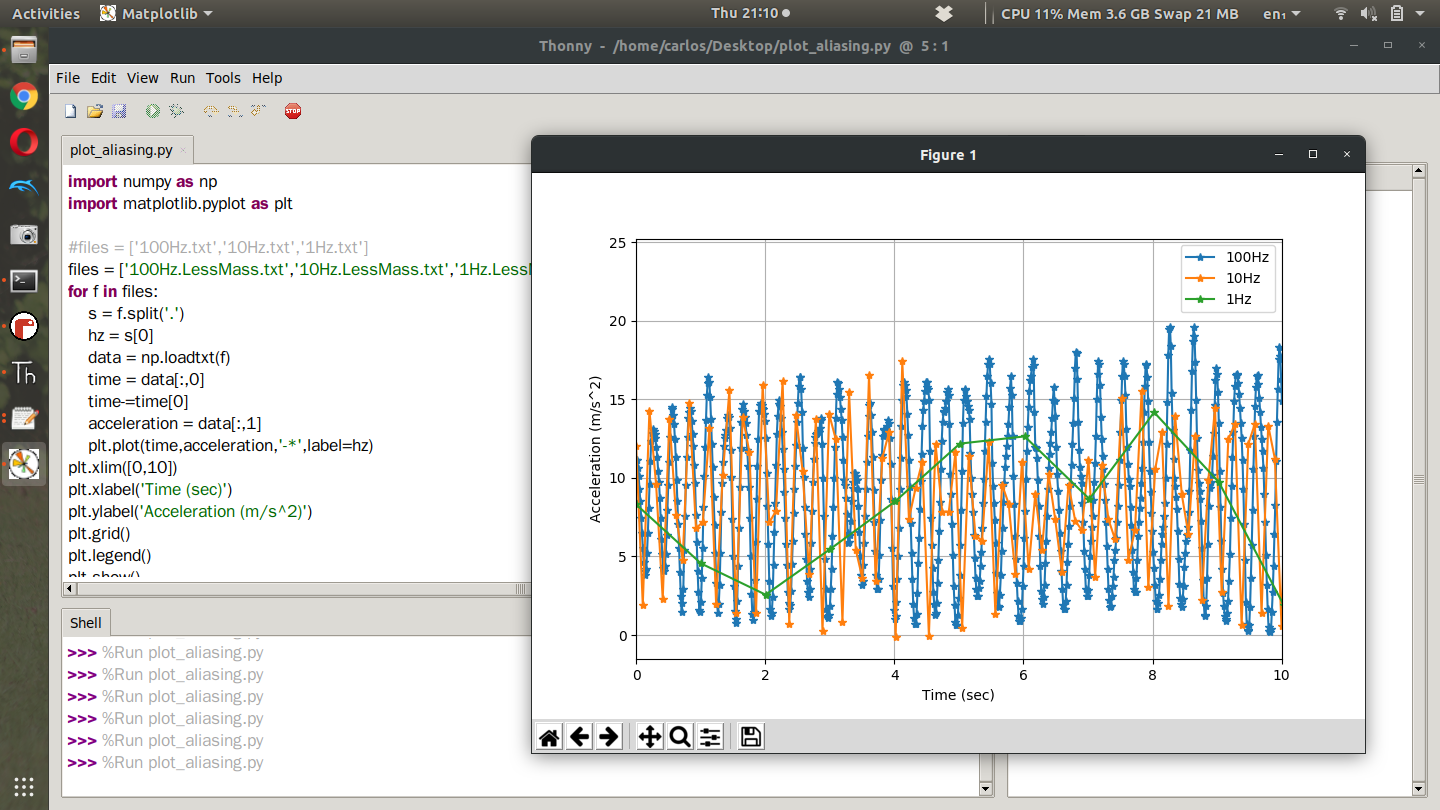
\includegraphics[width=\textwidth]{Figures/aliasing2.png}
  \end{center}
\end{figure}
In this case you can see that there were 33 cycles in 10 seconds which is 3.3 Hz. The Nyquist criteria states that I need to sample at 6.6 Hz. The Nyquist criteria is very specific though in that if you sample at twice the frequency, you will just obtain the correct frequency. This does not mean that you will capture every data point properly. Hence in the chart above, the blue line at 100 Hz is perfect, the green line at 1 Hz is too slow (less than 6.6 Hz) and the orange line at 10 Hz captures the frequency correctly but between 5 and 8 seconds does not adequately capture the waveform. In my opinion, in order to sample the data effectively and not just obtain the frequency of the waveform, you need to sample at 4 times the natural frequency. So for the waveform of 3.3 Hz, the Montalvo frequency would be 13.2 Hz which is higher than the 10 Hz. This explains why the 10 hz sample is not perfect while the 100 hz sample rate is much better. 

\subsection{Assignment}

For this assignment you are to create a system that oscillates and capture data while oscillating. You are to sample the system at 1, 10 and 100 Hz and plot the shifted and cleaned data for all 3 sample rates on the same graph. For the data sampled at 100 Hz you are then to estimate the initial amplitude, the settling time  and the period using the graph. Then compute the natural frequency and damping ratio. Finally, using equation \ref{e:secondorder}, plot the amplitude as a function of time on top of your 100hz sampled data. {\bf Note, if you decide to make a pendulum you must ensure that the CPX/CPB does not spin when oscillating otherwise you won't be able to use your acceleration data easily.}

Once you've completed the project above, upload a PDF with all of the photos and text
below included. My recommendation is for you to create a Word document
and insert all the photos and text into the document. Then export the
Word document to a PDF. For videos I suggest uploading the videos to
Google Drive, turn on link sharing and include a link in your
PDF. Note that all code must be included in the appendix or you'll be
penalized 10\%. 


\begin{enumerate}[itemsep=-5pt]
\item Include a photo of your experiment and explain the state that you are measuring - 10\%
\item Plot the results of your data (make sure to connect your data points) vs time for all 3 sampling frequencies (1,10, 100Hz) and include a legend - 20\%
\item Include a table of your estimated parameters as well as the natural frequency and damping ratio - 20\% 
\item Plot your measured data sampled at 100hz with your fitted equation on top - 20\%
\item Based on your results and your computed natural frequency, comment on the Nyquist frequency and the Montalvo frequency of your system and whether or not you encountered aliasing in your experiment based on the figures and the Nyquist/Montalvo frequency - 10\%
\end{enumerate}
